\documentclass[11pt]{article}
\usepackage{amssymb}
\usepackage[UTF8]{ctex}
\usepackage{geometry}
\usepackage{units}
\usepackage{pifont}
\geometry{
	a4paper,
	total={150mm,237mm},
	left=30mm,
	top=27mm,
	}
\usepackage{amsmath}
\usepackage{enumerate}
\usepackage{lipsum}
\usepackage{graphicx}
\usepackage{hyperref}
\usepackage{indentfirst}
\usepackage[graphicx]{realboxes}
\usepackage{booktabs}
\usepackage{cases}
\usepackage{subfig}  
\usepackage{float}
\usepackage{pythonhighlight}

\setlength{\parindent}{2em}
\title{HW7}
\author{姓名:陈锐林,学号:21307130148}

\begin{document}
\maketitle
\begin{large}
	\noindent Question1\\
\end{large}
\hspace*{2em}(1)可以看到,其指向正确的代码行。(2)它还告诉我产生冲突的地址和大小,如下图所示。
\begin{figure}[h]
    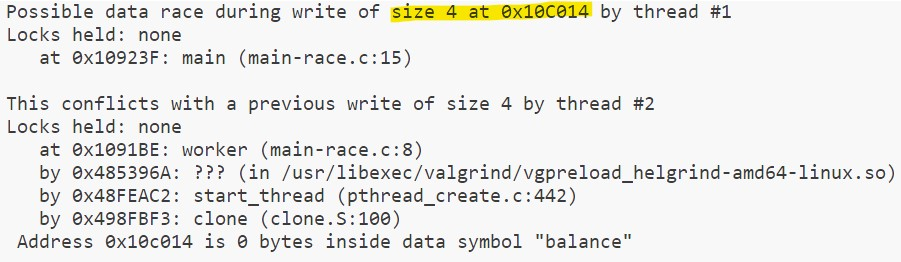
\includegraphics[width=11cm,height=4cm]{p7-1.jpg}
    \centering
\end{figure}\\
\begin{large}
	\noindent Question2\\
\end{large}
\hspace*{2em}(1)移走一行可能的冲突就不会报错了。(2)如果对两个地方都上锁,也不会有错误。(3)如果只对一个地方上锁,可能是会有错误的;但是helgrind并没有报告。\\

\begin{large}
	\noindent Question3\\
\end{large}
\hspace*{2em}在main-deadlock.c中,创建的两个线程都等待对方释放锁,最终会产生死锁。\\

\begin{large}
	\noindent Question4\\
\end{large}
\hspace*{2em}helgrind报告 lock order xxx violated,并在之后进行了进一步说明。
\begin{figure}[h]
    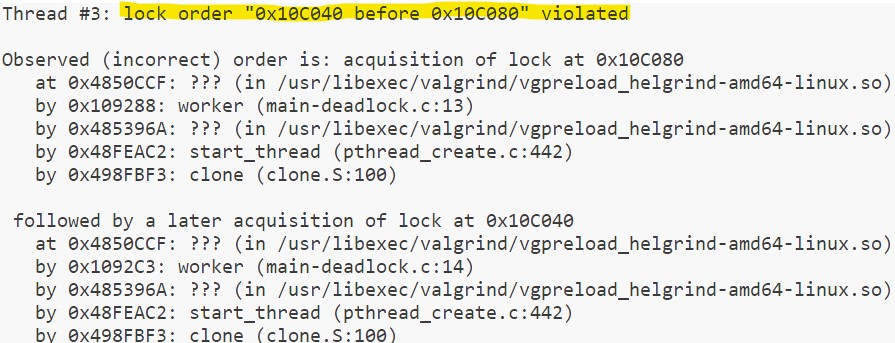
\includegraphics[width=11cm,height=5cm]{p7-2.jpg}
    \centering
\end{figure}\\
\newpage
\begin{large}
	\noindent Question5\\
\end{large}
\hspace*{2em}(1)在main-deadlock-global.c中,引入了第三个锁g,从理论上说,这时某个线程可以轻松地获得锁m1和m2,再释放;不应该出现问题。(2)但是helgrind仍然报告了lock order xxx is violated。(3)说明valgrind的这些工具仍然不是完美的,也是会有误解的。\\

\begin{large}
	\noindent Question6\\
\end{large}
\hspace*{2em}可以看到,在孩子进行时,父亲一直在循环中;这会导致效率不高,最后耗时多。\\

\begin{large}
	\noindent Question7\\
\end{large}
\hspace*{2em}(1)helgrind报告仍然可能会有数据竞争(如下图)。(2)这说明代码是有误的,报告指向了对于变量done的修改;说明这种方式既没效率也保证不了避免冲突。
\begin{figure}[h]
    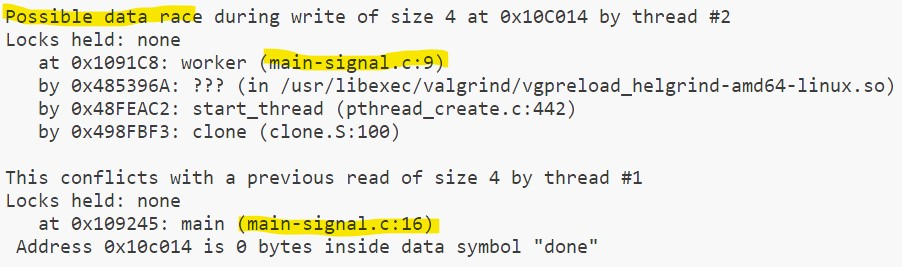
\includegraphics[width=11cm,height=5cm]{p7-3.jpg}
    \centering
\end{figure}\\

\begin{large}
	\noindent Question8\\
\end{large}
\hspace*{2em}(1)从正确性来说,两行内容是正确打印的,先后顺序正确(下图涂黄处)。(2)从表现来说,虽然之前的版本也能正确打印,但是两行文字隔了很远,中间有很多报错信息;最后总结处看出不带-cv版本有24个错,而现在的版本没有错误(下图涂绿处)。
\begin{figure}[h]
    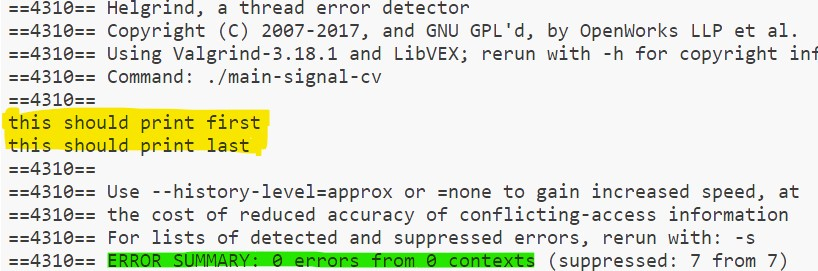
\includegraphics[width=11cm,height=5cm]{p7-4.jpg}
    \centering
\end{figure}\\

\begin{large}
	\noindent Question9\\
\end{large}
\hspace*{2em}再次运行 valgrind --tool=helgrind ./main-signal-cv,仍然没有报错。\\
\end{document}